\chapter{Digitální zpracování a reprodukce zvuku v embedded systémech}

\section{A/D a D/A převodníky}

Jakmile je docíleno převodu zvukové energie na energii elektrickou, dalším krokem může být konverze z analogové roviny do digitální. Pro opačný přechod se využívá \ac{DAC}. Audio Codec je poté označení pro ADC a DAC hardwarové komponenty dostupné v jednom pouzdře. Při rekonstrukci signálu z digitální do analogové podoby je důležité, aby signál splňoval Nyquistovu-Shannonovu vzorkovací podmínku. Ta hovoří o tom, že nejvyšší obsažená frekvence v původním pásmově omezeném signálu vynásobená dvěma by měla být menší než vzorkovací frekvence, protože ve spektru navzorkovaného signálu se kromě původního spektra nacházejí i jeho kopie posunuté o celočíselné násobky vzorkovací frekvence.
Lze vyjádřit vztahem
\begin{equation}
    f_s > 2f_{\max},
\end{equation}
kde $f_s$ je vzorkovací frekvence a $f_{\max}$ je nejvyšší frekvence původního signálu.
Při dodržení Nyquist-Shannonova teorému se kopie nepřekrývají, lze tak spektrum oddělit rekonstrukčním filtrem dolní propust a ze vzorků původní signál obnovit. Při nedodržení vzniká aliasing, jenž ani D/A převod ani rekonstrukční filtr nemohou odstranit \cite[s.~96--99]{smekal2023}. 
Filtry dolní propusti nejsou ideální a takřka žádné praktické využití nebude vzorkovat přesně na dvojnásobku, proto je jedna z často využívaných vzorkovacích frekvencí pro reprodukci hudby 44,1 kHz a ne 40 kHz \cite{katz2005embedded}.

\section{Delta-sigma D/A převodníky}

DAC převodníky lze rozdělit na dvě kategorie: ty pracující na Nyquistově vzorkovací frekvenci a převodníky s převzorkováním. Převodníky z první kategorie pracují s poměrem 1:1 vstupní ku výstupním vzorkům a každý vzorek je samostatně zpracován, bez ohledu na předchozí vzorky; jsou bezpamětné. 
Přivedením vstupního digitálního slova s bity $b_1$ až $b_N$ vede tedy na výstup
\begin{equation}
    U_{\mathrm{out}} = U_{\mathrm{ref}} \left( b_1 2^{-1} + b_2 2^{-2} + \cdots + b_N 2^{-N}, \right)
\end{equation}
kde $U_{\mathrm{ref}}$ je referenční napětí nezávislé na předchozím slově. Pro tento typ převodníků může být vzorkovací frekvence $f_{\mathrm{vz}}$ až na spodní hranici splnění Nyquistova kritéria. 
Technologický rozptyl parametrů (souběh, anglicky \textit{component matching, match\-ing ac\-cu\-ra\-cy}, vyjadřující jak přesně jsou si podobné součástky stejného typu a jmenovité hodnoty) je v praxi omezen asi na cca 0,02 \%. Tím pádem je ovlivněn i \ac{ENOB} na přibližně 12, ale mnoho audio zařízení vyžadují až 18 či 20 bitů. Takové Nyquistovy převodníky vyžadují více času, jsou pro zpracování audio signálu příliš pomalé.

Převzorkovací převodníky jsou schopny dosáhnout až 20 ENOB při vyšších rychlostech, využívají vzorkovací frekvenci 8krát až 512krát vyšší než je Nyquistova frekvence a výstup generují na základě předchozích hodnot (obsahují paměťové prvky). 

%----------------
%----------------
%----------------
Příkladem využití paměťových prvků je modulátor $\Delta\Sigma$ prvního řádu na obr.~\ref{fig:schema_delta_sigma} v základu tvořící akumulátor, dvouúrovňový kvantizátor a záporná zpětná vazba. Akumulátor uchovává svůj předchozí stav a přičítá k němu rozdíl mezi aktuálním vstupem a zpožděným výstupem modulátoru. Činnost uvedeného diskrétního modelu popisují vztahy
\begin{equation}
    \begin{aligned}
        y[n] &= y[n-1] + u[n] - v[n-1], \\
        v[n] &= Q\bigl(y[n]\bigr),
    \end{aligned}
    \label{eq:ds_model}
\end{equation}
kde $u[n]$ označuje vstupní signál, $y[n]$ stav
akumulátoru a současně vstup kvantizátoru,
$v[n]$ výstupní posloupnost a $Q(\cdot)$ kvantizační
funkci. Blok $z^{-1}$ představuje zpoždění
o jeden vzorek.

Zbytkovou chybu kvantování definujeme jako
\begin{equation}
    e[n] = y[n] - v[n].
    \label{eq:ds_chyba}
\end{equation}
Dosazením vztahu~\eqref{eq:ds_chyba}
do rovnic~\eqref{eq:ds_model} získáme
\begin{equation}
    v[n] = u[n] + e[n-1] - e[n].
    \label{eq:ds_vystup}
\end{equation}
Výstupní posloupnost tedy obsahuje vstupní signál
a diferenci kvantizační chyby. Tato diference
potlačuje nízkofrekvenční složky chyby, což představuje
princip jejího tvarování.

Odhad vstupního signálu vzniká digitální filtrací
výstupní posloupnosti. Význam průměrování lze ukázat
pro konstantní vstup $u[n]=u$. Průměr prvních $N$
výstupních vzorků je podle vztahu~\eqref{eq:ds_vystup}
roven
\begin{equation}
    \hat{u}_N
    = \frac{1}{N}\sum_{n=1}^{N} v[n]
    = u + \frac{e[0]-e[N]}{N}.
    \label{eq:ds_prumer}
\end{equation}
Při součtu se mezilehlé chybové příspěvky vzájemně
vyruší a zůstává pouze rozdíl počáteční a koncové
chyby. Pokud chyba zůstává ohraničená, odhad
$\hat{u}_N$ s rostoucím počtem vzorků konverguje
k hodnotě vstupu $u$. Hodnotu vstupního signálu
tak lze odhadnout průměrováním posloupnosti,
jejíž jednotlivé vzorky nabývají pouze dvou hodnot.

U časově proměnného vstupu je nutné volit vlastnosti
digitálního filtru s ohledem na požadovanou šířku
pásma signálu. Filtr klouzavého průměru na
obr.~\ref{fig:schema_delta_sigma} představuje jednoduchou
realizaci této výstupní filtrace.

%----------------
%----------------
%----------------

\begin{figure}[htbp]
    \centering
    \begin{tikzpicture}[
        scale=0.85,
        transform shape,
        >=Latex,
        thick,
        block/.style={
            draw,
            minimum width=16mm,
            minimum height=16mm
        },
        sum/.style={
            draw,
            circle,
            minimum size=5mm,
            inner sep=0pt
        },
        dot/.style={
            circle,
            fill,
            minimum size=3pt,
            inner sep=0pt
        }
    ]
        % Součtový uzel
        \node[sum] (s) at (0,0) {$+$};

        % Akumulátor
        \node[block, minimum width=24mm]
            (acc) at (2.4,0)
            {$\displaystyle\frac{1}{1-z^{-1}}$};

        % Kvantizátor
        \node[block] (q) at (5.8,0) {};

        % Výstupní odbočka
        \node[dot] (v) at (7.4,0) {};

        % Filtr klouzavého průměru
        \node[
            block,
            minimum width=30mm,
            align=center,
            font=\itshape
        ] (filter) at (9.9,0)
            {Moving\\Average\\Filter};

        % Zpoždění ve zpětné vazbě
        \node[
            draw,
            minimum width=12mm,
            minimum height=7mm
        ] (delay) at (2.4,-2.2) {$z^{-1}$};

        % Hlavní signálová cesta
        \draw[->] (-1.4,0) node[left] {$u$} -- (s.west);
        \draw[->] (s.east) -- (acc.west);
        \draw (acc.east) -- (q.west);
        \draw (q.east) -- (v);
        \draw[->] (v) -- (filter.west)
            node[midway, above] {$v$};
        \draw[->] (filter.east) -- ++(0.9,0)
            node[right] {$\hat{u}$};

        % Záporná zpětná vazba
        \draw (v) |- (delay.east);
        \draw[->] (delay.west) -| (s.south);
        \node at (0.48,-0.48) {$-$};

        % Symbol kvantizátoru
        \begin{scope}[shift={(q.center)}]
            \draw (-0.4,-0.6) -- (0,-0.6)
                -- (0,0.6) -- (0.4,0.6);
            \draw (-0.2,0) -- (0.2,0);
        \end{scope}
    \end{tikzpicture}

    \caption{Blokové schéma modulátoru $\Delta\Sigma$
        prvního řádu s filtrem klouzavého průměru.}
    \label{fig:schema_delta_sigma}
\end{figure}




\newpage
- Převzorkování

- delta sigma modulace, tvarování kvantizačního šumu 

- d/A převod a výstupní dolní propust

\section{PCM}



Nejjedodušší digitální reprezentací signálu je \ac{PCM}; pro každou periodu vzorkování je analogová amplituda zakódována s příslušnou digitální úrovní. 





\subsection{Digitalizace zvuku}

\subsection{Formáty audio souborů}

\subsubsection{Formát souboru WAV}

Formát WAV (\textit{Waveform Audio File Format}) je založen na kontejnerovém
formátu RIFF (\textit{Resource Interchange File Format}). Soubor ve formátu
RIFF se skládá z jednotlivých bloků označovaných jako \textit{chunks}.
Každý blok je identifikován čtyřznakovým identifikátorem FOURCC
(\textit{Four-Character Code}).

V případě běžného nekomprimovaného PCM WAV souboru se struktura skládá
z hlavičky RIFF a následných bloků \texttt{fmt} a \texttt{data}.
Zde je základní struktura hlavičky RIFF:
\ref{tab:wav_riff_header}.

\begin{table}[ht]
    \centering
    \caption{Struktura hlavičky RIFF souboru WAV}
    \label{tab:wav_riff_header}
    \begin{tabular}{lccc}
        \toprule
        \textbf{Pole} & \textbf{Offset [B]} & \textbf{Velikost [B]} & \textbf{Význam} \\
        \midrule
        \texttt{ChunkID}   & 0 & 4 & ASCII řetězec \texttt{RIFF} \\
        \texttt{ChunkSize} & 4 & 4 & Velikost souboru bez prvních 8 bajtů \\
        \texttt{Format}    & 8 & 4 & ASCII řetězec \texttt{WAVE} \\
        \bottomrule
    \end{tabular}
\end{table}

Pole \texttt{ChunkID} obsahuje posloupnost znaků \texttt{RIFF}, odpovídající bajtům \texttt{52 49 46 46}. Pole \texttt{ChunkSize}
udává velikost zbývající části RIFF bloku, tedy v případě základního
WAV souboru velikost celého souboru zmenšenou o 8 bajtů. Pole
\texttt{Format} obsahuje identifikátor \texttt{WAVE}.

Za hlavičkou RIFF následuje blok \texttt{fmt}, popisující formát uložených zvukových dat. Jeho struktura pro nekomprimovaný PCM signál je uvedena v tabulce \ref{tab:wav_fmt}.

\begin{table}[ht]
    \centering
    \caption{Struktura bloku \texttt{fmt } pro PCM WAV}
    \label{tab:wav_fmt}
    \begin{tabular}{lccp{7cm}}
        \toprule
        \textbf{Pole} & \textbf{Offset [B]} & \textbf{Velikost [B]} & \textbf{Význam} \\
        \midrule
        \texttt{Subchunk1ID}
        & 12 & 4
        & ASCII řetězec \texttt{fmt } \\

        \texttt{Subchunk1Size}
        & 16 & 4
        & Velikost zbývající části bloku; pro PCM je rovna 16 B \\

        \texttt{AudioFormat}
        & 20 & 2
        & Formát zvukových dat; hodnota 1 označuje PCM \\

        \texttt{NumChannels}
        & 22 & 2
        & Počet zvukových kanálů; 1 pro mono, 2 pro stereo \\

        \texttt{SampleRate}
        & 24 & 4
        & Vzorkovací frekvence v Hz, například 48\,000 Hz \\

        \texttt{ByteRate}
        & 28 & 4
        & Počet bajtů za sekundu \\

        \texttt{BlockAlign}
        & 32 & 2
        & Počet bajtů jednoho vzorkovacího rámce \\

        \texttt{BitsPerSample}
        & 34 & 2
        & Bitová hloubka jednoho vzorku \\
        \bottomrule
    \end{tabular}
\end{table}

Hodnota pole \texttt{ByteRate} je určena vztahem

\begin{equation}
    \texttt{ByteRate}
    =
    \texttt{SampleRate}
    \cdot
    \texttt{NumChannels}
    \cdot
    \frac{\texttt{BitsPerSample}}{8}.
\end{equation}

Podobně lze velikost jednoho vzorkovacího rámce vyjádřit jako

\begin{equation}
    \texttt{BlockAlign}
    =
    \texttt{NumChannels}
    \cdot
    \frac{\texttt{BitsPerSample}}{8}.
\end{equation}

Vzorkovací rámec zde představuje vzorky všech kanálů náležející ke
stejnému okamžiku vzorkování. Například u 16bitového stereofonního
signálu má jeden rámec velikost 4 B.

Za blokem \texttt{fmt } se v základní podobě PCM WAV souboru nachází
blok \texttt{data}, který obsahuje vlastní zvuková data.

\begin{table}[ht]
    \centering
    \caption{Struktura bloku \texttt{data}}
    \label{tab:wav_data}
    \begin{tabular}{lccp{7cm}}
        \toprule
        \textbf{Pole} & \textbf{Offset [B]} & \textbf{Velikost [B]} & \textbf{Význam} \\
        \midrule
        \texttt{Subchunk2ID}
        & 36 & 4
        & ASCII řetězec \texttt{data} \\

        \texttt{Subchunk2Size}
        & 40 & 4
        & Počet bajtů zvukových dat \\

        \texttt{Data}
        & 44 & proměnná
        & Jednotlivé vzorky zvukového signálu \\
        \bottomrule
    \end{tabular}
\end{table}

Velikost datové části lze pro PCM signál vyjádřit jako

\begin{equation}
    \texttt{Subchunk2Size}
    =
    N_\mathrm{samples}
    \cdot
    \texttt{NumChannels}
    \cdot
    \frac{\texttt{BitsPerSample}}{8},
\end{equation}

kde $N_\mathrm{samples}$ představuje počet vzorků jednoho kanálu.

Vícebajtové číselné hodnoty jsou ve standardním WAV souboru ukládány v pořadí \textit{little-endian}. Například 32bitová hodnota \texttt{0x12345678} je tedy v souboru uložena jako posloupnost bajtů \texttt{78 56 34 12}. Čtyřznakové identifikátory, například \texttt{RIFF}, \texttt{WAVE}, \texttt{fmt } nebo \texttt{data}, jsou naproti tomu ukládány přímo jako posloupnost ASCII znaků\cite{wav_internet_archive}.

\subsubsection{Načítání WAV do STM32}
https://www.phippselectronics.com/how-to-play-a-wav-file-on-stm32/
% --------------------------------------------------
% --------------------------------------------------



\subsection{D/A převodníky}
Princip Delta Sigma modulace

Převzorkování

I2S rozhraní

SAI rozhraní
    - Circular Linked-List nastavení v STM32, pro přenos SAI je vhodný 2 slovný FIFO


\section{Koncepce návrhu}

Obhajova výběru komponent

\subsection{Mikrokontrolér a práce v CubeIDE}
Proč zrovna to

Dostatek RAM a FLASH paměti

\subsection{Audio řetězec}
\subsubsection{D/A převodník PCM5102A}
typické zapojení podle datasheetu 

\begin{figure}[htbp]
    \centering
    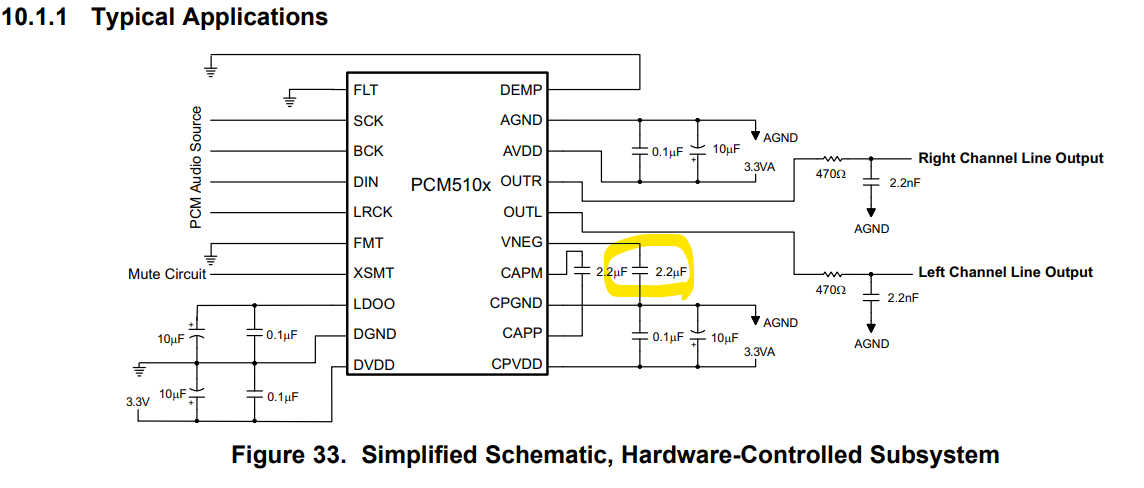
\includegraphics[width=0.8\textwidth]{obrazky/PCM5102A_typical_application.png}
    \caption{Typické zapojení PCM510x}
    \label{fig:PCM5102A_typical_application}
\end{figure}

Obsahuje integrovanou nábojovou pumpu - vytváří záporné napájecí napětí přestože je čip krmen 3,3 V. DAC má pak soustředěný výstup kolem 0V.
Ale je zapotřebí přidat kondenzátor mezi CAPP a CAPM piny (2 a 4, používá se pro přenos náboje), a potom ještě jeden mezi VNEG a CPGND piny (5 a , filtruje vztvořené záporné napětí).

PIN 10 DEMP na GND, vypne se tam de-emphasis.

PIN 11 FLT na GND, takže je použít normální FIR filtr.

PIN 12 SCK na GND, takže je použít interní PLL bez externího MCLK

PIN 16 FMT na GND, jde o standardní I2S formát.

PIN 17 XSMT, připojen na 3,3V.


- Čip využívá Direct Path, nepotřebuje na audio výstupu oddělovací kondenzátory, protože výstup už kmitá kolem nuly (GND). Ale aby toho byl schopen dosáhnout pomocí napětí +3,3 V, musí si vytvořit i záporné napětí -3,3 V (VNEG větev). C22 mezi piny CAPP a CAPM (flying capacitor), má dvě fáze. V první fázi se nabije na 3,3 V, ve druhé fázi se přepne mezi GND a pin VNEG (přelije náboj do záporné větve). - Hodnota převzaná od Texas Instruments.

- C23 mezi VNEG a CPGND je vyhlazovací kondenzátor záporného napětí, udržuje stabilních 3,3 V. 

- C24 - analogový výstupní filtr RC

- C25 - analogový výstupní filtr RC

- C26 - nízká parazitní indukčnost, odvádí ryché proudové špičky - doporučeno TI

- C27 - dobrý na pomalejší změny odběru proudu - doporučeno TI

- C28 (100 nF, potlačuje rychlé rušení vznikající při spínání nábojové pumpy) a C29 (10 uF, stabilizuje 3,3 V napájení) - protože pin CPVDD odebírá proud v pulzech, pulzy mohou vytvoři rušení - hodnoty převzaté z doporučení Texas Instruments.

- C30 a C 31 - stejně jako u C26 a C27.

- C32 - filtrace a stabilizace interního LDO (interního napěťového regulátoru, vytářející cca 1,8 V z 3,3 V pro )

- C33 - filtrace vf 

\subsubsection{Výstupní analogový filtr RC}

- kondenzátory C24, C25 filtrují vf složky pro každý kanál do země -> filtr dolní propust
- aby filtr neovlivnil amplitudu/fázi slyšitelných vyšších tónů, volí se mezní frekvence 7 krát až 10 krát vyšší než 20 kHz. Hlavně je zapotřebí vyfiltrovat frekvence v MHz
- hodnoty rezistory C22 a C23 jsou natolik nízké, že neovlivní úbytek sigálu na vstupní impedanci běžného koncového zesilovače.

$ f_c = \frac{1}{2\pi R C} = \frac{1}{2\pi \cdot 470 \cdot 2{,}2 \cdot 10^{-9}} \approx 154 kHz$

\subsubsection{Sluchátkový zesilovač TPA6111A2D}
Zesílení analogového stereofonního signálu z D/A převodníku PCM5102A je docíleno pomocí integrovaného sluchátkového zesilovače TPA6111A2D od Texas Instruments. Obvod obsahuje dva nezávislé zesilovací kanály v invertujícím zapojení, umožňuje provoz při 3,3 V. 

Zesílení jednotlivých kanálů je určeno poměrem zpětnovazebního rezistoru $R_F$ a vstupního rezistoru $R_I$, platí vztah 
$A_v=-\frac{R_F}{R_I}$, kde pro $R_F$ i $R_I$ jsou zvoleny hodnoty 20 kohm, tedy $A_v=-\frac{20 komh}{20 kohm}=-1$. Napěťové zesílení se tedy rovná jedné, rovno zesílení 0 dB, nedochází k změně amplitudy. Záporné znaménko zde vyjadřuje fázovou inverzi o 180 stupňů. Zvolená konfigurace odpovídá doporučenému zapojení uvedené v technické dokumentaci dané součástky.

Ekvivalentní odpor působící na invertující vstup zesilovače je dán paralelní kombinací $R_F$ a $R_I$, $R_{\mathrm{eq}}=\frac{R_F R_I}{R_F+R_I}
=10,\mathrm{k}\Omega$, tato hodnota je v rámci doporučení výrobcem, tedy od 5 kOhm do 20 kOhm.

Při návrhu bylo zohledněno rozdílné napěťové rozmezí výstupních signálů D/A převodníku a sluchátkového zesilovače. Převodník PCM5102A při plném vybuzení dosahuje výstupní úrovně 2,1 V RMS (5,94 V špička špička, mnohem více, než zesilovač dokáže reprodukovat bez zkreslení). Regulace hlasitosti bude proto řícena digitálním útlumem PCM vzorků v mikrokontroléru STM32. Maximální úroveň bude stanovena s ohledem na výstupní napěťový rozkmit zesilovače, s ohledem na impedanci připojených sluchátek\dots

Ostatní komponenty ve schématu okolo TPA6111A2D

Vstupní vazební kondenzátory C38 a C39 (1 µF), sériově zapojeny mezi výstupy D/A převodníku a vstupy zesilovače, oddělující stejnosměrné složky signálu. Společně se vstupními rezistory R24 a R26 vytváření RC filtr horní propusti, určující dolní mezní kmitočet přenosové charakteristiky = 8 Hz.

\begin{equation}
    f_c = \frac{1}{2\pi R_I C_I}
    = \frac{1}{2\pi \cdot 20 \times 10^3 \cdot 1 \times 10^{-6}}
    \approx 7{,}96\,\mathrm{Hz}
    \label{eq:mezni_frekvence_vstup}
\end{equation}

Kondenzátor C34 o kapacitě 1 uF, ovlivňuje časový průběh náběhu interního předpětí, čímž omezuje vznik nechtěných impulzů při zapnutí zesilovače.

Blokovací kondenzátory C37 (potlačující vysokofrekvenční rušení a rychlé napěťové přechody), C40, zlepšují stabilitu napájení a omezují nežádoucí vlivy napájecího rušení na výstupní audio signál.
\begin{equation}
    X_C = \frac{1}{2\pi f C}
    \label{eq:kapacitni_reaktance}
\end{equation}
S rostoucí frekvencí klesá kapacitní reaktance, kondenzátor představuje pro vf složky nízkoimpedanční cestu ke GND. 

Výstupní vazební kondenzátory C17, C18 polarizované elektrolytické, zabraňují průchodu stejnosměrné složky do připojených sluchátek. Zvolená kapacita 470 µF pro sluchátka o impedanci 32 Ohm odpovídá dolní mezní frekvenci 10,58 Hz, podle 
\begin{equation}
    f_c = \frac{1}{2\pi R_L C_{\mathrm{out}}}
    = \frac{1}{2\pi \cdot 32 \cdot 470 \times 10^{-6}}
    \approx 10{,}58\,\mathrm{Hz}
    \label{eq:mezni_frekvence_vystup}
\end{equation}


\subsection{Periferie}
SD karta
    



displej

\subsection{Napájení}

\ac{LiPo} - vybíjecí charakteristiky?

Power Path

\section{Realizace Hardware části práce}

\subsection{Schéma zapojení napíjecí části}

\subsection{Schéma zapojení analogové audio části}
Výpočet součástek kolem čipu PCM5102A

Výpočet součástek kolem čipu TPA6111A2D

    - zpětnovazební rezistory pro zisk

    - výpočet dolního mezního kmitočtu vstupních a výstupních kondenzátorů

\subsection{Návrh PCB desky}

Rozmístění součástek po desce




